% Chapter 2

\chapter{Convolutional Neural Networks} % Main chapter title

\label{Chapter2}

%-------------------------------------------------------------------------------
%-------------------------------------------------------------------------------

\section{CNNs: Layer by Layer}

Convolutional neural networks have been very successful in computer vision as their key ingredient convolution filters preserve 2D structure and are able to pull features from images. Back propogation and stochastic gradient descent are used to optimize these filters in order to produce. Here I will cover some of the most common layers used in CNNs.

\subsection{Convolution Layer}

The first and foremost layer is the convolution layer. A convolution layer contains a set of filters which are \textit{convolved} across feature maps in order to get the feature map. Let's take a concrete look at what this means. Imagine we are working with images that are of the shape 28x28x3 pixels. We then decide we want to use a convolution filter of size 2x2x5 which will result in a 28x28x5 feature map. Each kernel in this filter will be of size 2x2x3 since the depth in our original image is 3 and there will be five kernels. We then take the dot product of each slice in our 2x2x3 matrix against the original image at pixel 0x0 giving us 3 scalar values which are summed to get the first value in the first feature map of the output. We then slide these filters across the entire feature map in x and y thereby creating a new feature map.  See ~\ref{fig:Convolution} for an example of convolving two 3x3x3 kernels on a 7x7 image.  A few things to consider when sliding the feature maps are image padding. For pixel 0,0 in our example part of the filter would be off the image. To keep the convolution consistent people will often times pad the edges of the image with 0 or 0.5. Additionally a stride length can be set which determines how far we move the filter at each step. A stride length of 2 would skip every other pixel when sliding.

\begin{figure}[ht]
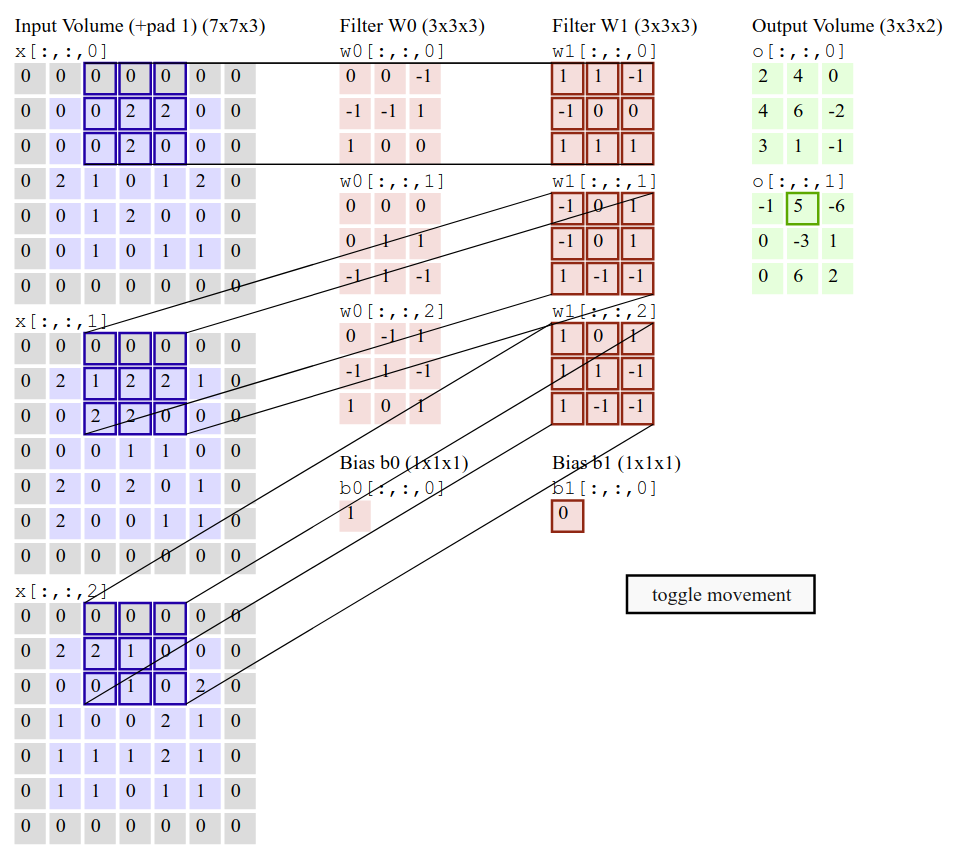
\includegraphics[width=0.9\textwidth]{Figures/Convolution.png}
\caption{An example of performing a 3x3 convolution with a depth of two on an 7x7x3 image with 1 pixel of padding from Andrej Karpathy's Stanford CNN Course \cite{StanfordConv}}
\label{fig:Convolution}
\end{figure}

\subsection{Activation Layer}

Its common after each of the convolutional layers to apply a non-linear activation function. A few examples of activation include: \\

\[ \sigma(x) = \frac{1}{1+e^{-x}} \]
\[ \tanh(x) = \frac{e^x - e^{-x}}{e^x + e^{-x}} \]

\[ ReLu(x) = \begin{cases}
      0 & x < 0 \\
      x & x \geq 0
   \end{cases}
\]

ReLu or rectified linear unit has been a popular choice for cnns as it is computation efficient without sacrificing accuracy.

\subsection{Pooling Layer}

Pooling layers are used to downsample feature maps from layer to layer. Two common flavors of pooling layers are max pooling and average pooling. Max pooling simply looks at a window and returns only the maximum value. Average pooling as it names suggests averages all the values in the window and returns that value. Lets take for example a 2x2 max pooling layer with an feature map of size of 128x128x32. After applying the pooling layer we would have 64x64x32 as an output. A common intuition behind max pooling is that it provides spatial invariance, i.e. if an object shifts by a few pixels we will still have a high response. An alternative to max pooling is using strided convolutions. The argument for this is that a good amount of information is lost in pooling layers.

\subsection{Fully Connected Layer}

Fully connected layers are what we traditional think of as the multi-layer perceptron model. They are commonly used in the final layer of CNNs to distill feature maps from a multi-dimensional matrix into a vector that can be then used for classification or regression. As a simple example are classification networks that will use two fully connected layers where the output is a vector of the same length as number of classes they want to predict from. SoftMax is applied to the vector to normalize the sum of the vector to one and then each scalar in the vector is interpreted as a likelihood of that image being of that particular class.

\subsection{Transfer Learning}

Transfer learning is the process of taking a neural network trained for a certain task and refining it for another. A common example of this is retraining a classification network to predict a different set of classes than what it was originally trained for or changed from a classifier to a regression network. The common intuition for this is that the early layers in the network have learned basic features like, curves, corners, or other simple patterns that are universal in all types of objects. The top layers which carry the strong semantic information are closer to the end and therefore receive more gradient during back propagation. Some methods even freeze the weights for lower levels as fixed feature extractors and only allow the the final layers to change during training. As a bonus, transfer learning reduces the total time to train a network as the lower levels of a network take longer to train that the deeper layers.

When exploring new architectures it is common procedure to simply download a set of weights for a popular network backbone and just apply transfer learning from there. In these next sections I will cover some of the popular network backbones.

\subsection{VGG16}

VGG16 was one of the first major networks after AlexNet which went for simplicity and depth \cite{VGG16}. The first contribution was its simplicity. CNNs before VGG used very large filter sizes, for example AlexNet used 11x11, which led to large parameter sizes. The authors of VGG16 instead used series of two back to back convolution/ReLu layers with 3x3 filters before doing max pooling. VGG16 at the time was considered a very deep network with 13 convolution layers and 3 fully connected layers. It showed that very deep networks were extremely important in learning the hierarchical features necessary for good classification. VGG16 scored $7.3\%$ error rate on ImageNet dataset.

\subsection{ResNet}

In 2015 Microsoft Research came out with \textit{Deep Residual Learning for Image Recognition} \cite{ResNet} which had 152 layers and new type of of block called the residual block. It scored $3.6\%$ on the ImageNet challenge in 2015. A residual block is a normal feed forward neural network that adds in \textit{shortcut} connections where the input to a layer is both fed through a layer but also routed around the layer and added to the output of the next layer. See ~\ref{fig:ResBlock} for a visual description. They hypothesized that a residual mapping induced by this block would be easier to learn than the original feed-forward network. ResNets come in several popular forms now such as ResNet18, ResNet32, ResNet50, ResNet101, and ResNet152, where the choice of depth is based on computational resources and dataset. Most popular deep learning frameworks have pretrained ResNet models available for download.

Another intuition behind ResNets success is that the \textit{shortcut} connections allow gradients to move more easily through the network which helps alleviate a problem known as the vanishing gradient. Vanishing gradients is the problem where the loss at the end of the network has very little impact on changing the weights on the earlier layers and was one of the main reasons preventing networks from going as deep as ResNet. In the next network the use of skip connection is taken even further.

\begin{figure}[ht]
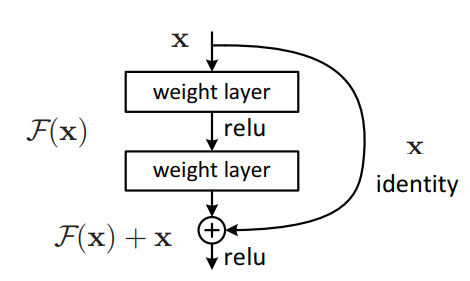
\includegraphics[width=0.9\textwidth]{Figures/ResBlock.png}
\caption{Diagram of Residual Block from \cite{ResNet}}
\label{fig:ResBlock}
\end{figure}

\subsection{DenseNet}

In 2016 Densely Connected Convolutional Networks (DenseNets) were proposed and shown to match and beat the residual network architecture on many datasets while using much fewer parameters and therefore computation. With DenseNets the authors connect all feature maps of same size together through concatenation so that the lth layer will have (l-1) feature maps. This is different then the ResNet model which uses summation in its shortcut connections. In order to concatenate feature maps across max pooling layers DenseNet introduce transition layers. These transition layers pass the prior feature maps through batch normalization, convolution, and finally average pooling before concatenating them to layers further down.

\begin{figure}[ht]
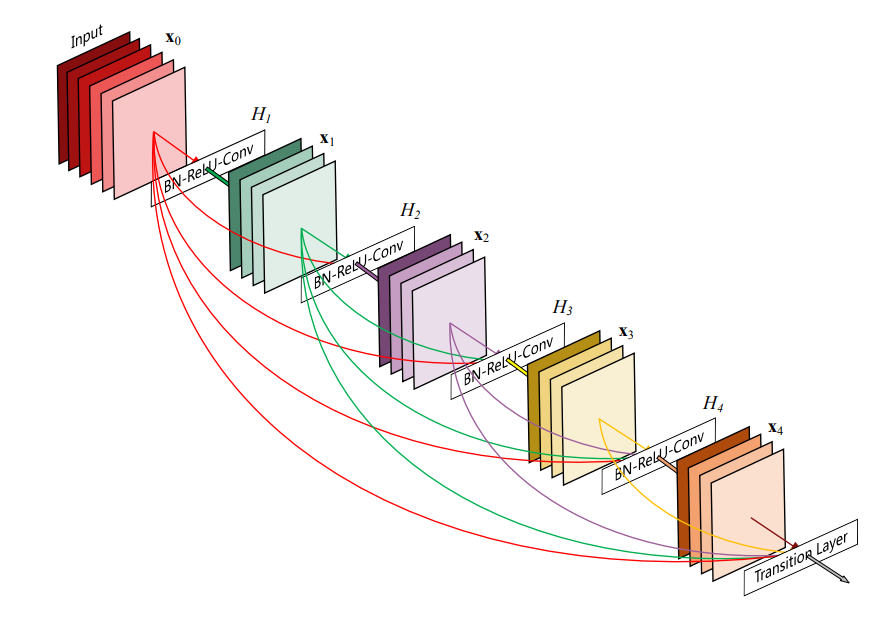
\includegraphics[width=0.9\textwidth]{Figures/DenseNet.png}
\caption{Diagram of Residual Block from \cite{DenseNet}}
\label{fig:DenseNet}
\end{figure}

%-------------------------------------------------------------------------------
%-------------------------------------------------------------------------------
\section{Object Detection Networks}

Object detection networks deal with the problem of first localizing an object with an image frame as well as classifying that object and is generally considered a harder problem then pure classification tasks. The two popular datasets for benchmarking results are \textit{Common Objects in Context} (COCO) \cite{COCO} and \textit{The PASCAL Visual Object Classes} (PASCAL VOC) \cite{VOC}. At the time this work began the two most popular object detection networks were Faster-RCNN and YOLOv2 which I will cover in depth in the next two sections. Since then the state of the art has progressed considerably. Future work might include exploring this architectures.

\subsection{Faster-RCNN}

Faster-RCNN \cite{FASTER-RCNN}, where the R stands for region, is one of the most popular object detection networks at the moment and is an advancement on the authors previous two networks RCNN and Fast RCNN. The authors show results for both VGG16 and ZF network backbones, but many open source implementations of Faster-RCNN have replaced these backbones with various ResNet and DenseNets backbones.

The main contribution of Faster-RCNN is the Region Proposal Network (RPN) which replaces Fast-RCNNs slower, more complicated region proposal mechanism. It works by sliding a window across the final convolution feature map in a network and simultaneously predicting class probability and objectness. Objectness in this context is the probability that there is an object present in the bounding box. The RPN is implemented as a single NxN conv layer that maps into a lower dimension followed by two 1x1 conv layers for class probability and objectness. Furthermore they make use anchor boxes or priors on bounding boxes to make the task of the box regressor easier. At each position in the sliding window there are 9 anchor boxes which the regressor predicts bounding boxes with respect to.

The training scheme for this network is a multi-step process which involves training the RPN and Fast-RCNN networks separately and then later fixing the conv layers of Fast-RCNN and just fine-tuning the RPN.

\subsubsection{Loss}
The loss for Faster-RCNN is split into two parts as shown below.

\begin{align}
    \Loss = \Loss_{cls} +\Loss_{reg}
\end{align}

Given $p_i$ is the predicted confidence that the ith anchor box is an object and $p_i^*$ is a binary indicator that the anchor box has an IoU greater than 0.7 with a ground truth we can define the loss as:

\begin{align}
    \Loss_{cls}(p_i,p_i^*) = \frac{1}{N_{cls}} \sum_{i=1}^{A} [p_i\log(p_i) + (p_i^*-p_i)\log(1-p_i)]
\end{align}

We then parameterize the anchor box and bounding box truth as the following where $_a$ indicates a parameter from the anchor box and $*$ from the ground truth.

\begin{align}
    t_x = \frac{(x - x_a)}{w_a} \\
    t_y = \frac{(y - y_a)}{h_a} \\
    t_w = \log(\frac{w}{w_a}) \\
    t_h = \log(\frac{h}{h_a}) \\
    t_x^* = \frac{(x^* - x_a)}{w_a} \\
    t_y^* = \frac{(y^* - y_a)}{h_a} \\
    t_w^* = \log(\frac{w^*}{w_a}) \\
    t_h^* = \log(\frac{h^*}{h_a}) \\
\end{align}

Next we define the regression loss where again we use $p_i^*$ as an indicator whether this anchor box has an IoU above 0.7 with the ground truth.

\begin{multline}
    \Loss_{reg}(p_i^*, t, t^*) = p_i^*(Smooth_{L1}(t_x-t_x^*) + Smooth_{L1}(t_y-t_y*) \\ + Smooth_{L1}(t_w-t_w*) + SL1(t_h-t_h*)) \\
\end{multline}

\begin{align}
    Smooth_{L1}(d) = \begin{cases}
      0.5d^2 & if |d| \leq 0 \\
      |d| - 0.5 & otherwise
   \end{cases}
\end{align}

\subsection{YOLOv2}

YOLOv2, You Only Look Once, is another successful object detector released in 2016 \cite{YOLOv2}. It's key contribution is a unified network that simultaneously predicts object class and location with out the use of a secondary Region Proposal Network. While maintaining comparable accuracy to Faster-RCNN it runs at a much higher frame rate.

The backbone is of the authors design that uses only 3x3 and 1x1 convolutions, max pooling layers, and batch normalization. The network contains 23 convolution layers, 5 max pooling layers, and one short cut layer that concatenates features from lower levels to the final layer. Since the model contains no fully connected layers the network input size is unconstrained. The 5 max pooling layers of stride 2 mean that the final feature map will have a width and height that is the original width and height divided by $2^5$. As such the the original network input is usually selected to be a multiple of 32 i.e. 320, 416, 608, etc... An example of the network architecture is shown in table~\ref{table:YOLOV2}

\begin{center}
\begin{table}[h]\footnotesize
    \caption{YOLOv2 Network Architecture layer by layer for an input resolution of 608 x 608}\label{table:YOLOV2}
    \begin{tabular}{| l | l | l | l | l |}
    \hline
    layer  & filters & size & input & output \\ \hline \hline

    \rowcolor{LightCyan}
    0 conv & 32 & 3 x 3 / 1 & 608 x 608 x 3 & 608 x 608 x 32 \\ \hline

    \rowcolor{Salmon}
    1 max  & N/A & 2 x 2 / 2 & 608 x 608 x  32   &  304 x 304 x  32 \\ \hline \hline

    \rowcolor{LightCyan}
    2 conv &       64  & 3 x 3 / 1   & 304 x 304 x  32   & 304 x 304 x  64 \\ \hline

    \rowcolor{Salmon}
    3 max &     N/A     & 2 x 2 / 2   & 304 x 304 x  64   &   152 x 152 x  64 \\ \hline \hline

    \rowcolor{LightCyan}
    4 conv &    128  & 3 x 3 / 1   & 152 x 152 x  64   &   152 x 152 x 128 \\ \hline

    \rowcolor{LightCyan}
    5 conv &     64  & 1 x 1 / 1   & 152 x 152 x 128   &   152 x 152 x  64 \\ \hline

    \rowcolor{LightCyan}
    6 conv &    128  & 3 x 3 / 1   & 152 x 152 x  64   &   152 x 152 x 128 \\ \hline

    \rowcolor{Salmon}
    7 max &     N/A     & 2 x 2 / 2   & 152 x 152 x 128   &    76 x  76 x 128 \\ \hline \hline

    \rowcolor{LightCyan}
    8 conv &    256  & 3 x 3 / 1   &  76 x  76 x 128   &    76 x  76 x 256 \\ \hline

    \rowcolor{LightCyan}
    9 conv &    128  & 1 x 1 / 1   &  76 x  76 x 256   &    76 x  76 x 128 \\ \hline

    \rowcolor{LightCyan}
   10 conv &    256  & 3 x 3 / 1   &  76 x  76 x 128   &    76 x  76 x 256 \\ \hline

    \rowcolor{Salmon}
   11 max &     N/A     & 2 x 2 / 2   &  76 x  76 x 256   &    38 x  38 x 256 \\ \hline \hline

    \rowcolor{LightCyan}
   12 conv &    512  & 3 x 3 / 1   &  38 x  38 x 256   &    38 x  38 x 512 \\ \hline

    \rowcolor{LightCyan}
   13 conv &    256  & 1 x 1 / 1   &  38 x  38 x 512   &    38 x  38 x 256 \\ \hline

    \rowcolor{LightCyan}
   14 conv &    512  & 3 x 3 / 1   &  38 x  38 x 256   &    38 x  38 x 512 \\ \hline

    \rowcolor{LightCyan}
   15 conv &    256  & 1 x 1 / 1   &  38 x  38 x 512   &    38 x  38 x 256 \\ \hline

    \rowcolor{LightCyan}
   16 conv &    512  & 3 x 3 / 1   &  38 x  38 x 256   &    38 x  38 x 512 \\ \hline

   \rowcolor{Salmon}
   17 max &     N/A     & 2 x 2 / 2   &  38 x  38 x 512   &    19 x  19 x 512 \\ \hline \hline

    \rowcolor{LightCyan}
   18 conv &   1024  & 3 x 3 / 1   &  19 x  19 x 512   &    19 x  19 x1024 \\ \hline

    \rowcolor{LightCyan}
   19 conv &    512  & 1 x 1 / 1   &  19 x  19 x1024   &    19 x  19 x 512 \\ \hline

    \rowcolor{LightCyan}
   20 conv &   1024  & 3 x 3 / 1   &  19 x  19 x 512   &    19 x  19 x1024 \\ \hline

    \rowcolor{LightCyan}
   21 conv &    512  & 1 x 1 / 1   &  19 x  19 x1024   &    19 x  19 x 512 \\ \hline

    \rowcolor{LightCyan}
   22 conv &   1024  & 3 x 3 / 1   &  19 x  19 x 512   &    19 x  19 x1024 \\ \hline

    \rowcolor{LightCyan}
   23 conv &   1024  & 3 x 3 / 1   &  19 x  19 x1024   &    19 x  19 x1024 \\ \hline

    \rowcolor{LightCyan}
   24 conv &   1024  & 3 x 3 / 1   &  19 x  19 x1024   &    19 x  19 x1024 \\ \hline \hline

   \rowcolor{LightGreen}
   25 route  & 16 & N/A & N/A & N/A \\ \hline

   \rowcolor{Tan}
   26 reorg & N/A &            / 2      & 38 x  38 x 512    &    19 x  19 x2048 \\ \hline

   \rowcolor{LightGreen}
   27 route & 26 & 24 & N/A & N/A \\ \hline \hline

    \rowcolor{LightCyan}
   28 conv &   1024  & 3 x 3 / 1   & 19 x  19 x3072    &    19 x  19 x1024 \\ \hline

    \rowcolor{LightCyan}
   29 conv &     35  & 1 x 1 / 1   & 19 x  19 x1024    &    19 x  19 x  35 \\ \hline

    \hline
    \end{tabular}
\end{table}
\end{center}

YOLOv2 takes a simple approach to bounding box regression and class prediction. To understand how it works lets view the final feature map as a grid. At each location in this grid we want to predict bounding boxes and give a confidence metric for how likely there is to be an object there. We want to predict 5 numbers at each location in the grid plus a confidence for each class as show below:

\begin{align}\label{eq:bbox_regressed}
    t_x,t_y,t_w,t_h,t_o,P(C_1),...,P(C_N)
\end{align}

The parameters $t_x,t_y,t_w,t_h$ are regressed with relation to the feature map x,y location which we call $f_x$ and $f_y$. Further $t_x,t_y$ are constrained to be between [0,1] by the logistic function. We also define $p_w,p_h$ as the prior width and height for the anchor boxes.


\begin{align}
    b_x &= \sigma(t_x) + f_x \\
    b_y &= \sigma(t_y) + f_y \\
    b_w &= p_w * exp(t_w) \\
    b_h &= p_h * exp(t_h)
\end{align}

Like Faster-RCNN the author uses anchor boxes as priors for predicting bounding boxes at each locations. The author determined that 5 prior anchor boxes was a good trade-off between accuracy and efficiency. For each prior bounding box we need to predict the parameters shown in equation~\ref{eq:bbox_regressed}.

Lets take a concrete look at this with an example. Say that our input resolution is 416 x 416, we have 3 classes, and are using 5 prior anchor boxes. Dividing our input resolution by 32 we obtain our final feature map width and height equal to 13. Now at each location in this 13 x 13 map we need to regress 3 classes and 5 bounding box parameters for 5 anchor boxes.

\begin{align}
    (5 * (5 + 3)) * 13^2) = 6760
\end{align}

Instead of using a several fully connected layer to regress these numbers the author simply uses a 1x1 conv in the prior layer and sets the number of filters equal to the number of anchors multiplied by the 5 parameters plus the number of classes. In table~\ref{table:YOLOV2} there are 5 anchors and 2 classes meaning there are 35 filters going into the final feature map. Which can be seen on layer 29.

This setup allows the user to have the freedom to change the input resolution on the fly without having to modify the final layer. The only information we need a prior is the number of classes.

\subsubsection{Loss}

The loss function for YOLOv2 consists of 4 separate parts

\begin{align}
    \Loss_{YOLOv2} = \Loss_{coord} + \Loss_{obj} + \Loss_{noobj} + \Loss_{class} \\
\end{align}

The first part $\Loss_{coord}$ deals with bounding box regression.

\begin{multline}
    \Loss_{coord} = \lambda_{cood} \sum_{i=1}^{f_x*f_y} \sum_{j=i}^{Anchors}
    \indicator_{obj}^{i,j} [
        (\sigma(t_x^{(i,j)}) - \sigma(\hat{t}_x^{(i,j)}))^2 +
        (\sigma(t_y^{(i,j)}) - \sigma(\hat{t}_y^{(i,j)}))^2 + \\
        (\sigma(t_w^{(i,j)}) - \sigma(\hat{t}_w^{(i,j)}))^2 +
        (\sigma(t_h^{(i,j)}) - \sigma(\hat{t}_h^{(i,j)}))^2] \\
\end{multline}

The next part deal with the loss associated with predicting the objectness of the bounding box. Ideally we would like the objectness to predict the IoU of the predicted bounding box with the true bounding box. This is a little unintuitive as during inference we do not have access to the truth. The $\Loss_{noobj}$ is there to punish false positives.

\begin{align}
    \Loss_{obj} = \lambda_{obj} \sum_{i=1}^{f_x*f_y} \sum_{j=i}^{Anchors} \indicator_{obj}^{i,j} (IoU_{truth}^{pred} - \sigma(\hat{t}_o^{(i,j)}))^2 \\
    \Loss_{noobj} = \lambda_{noobj} \sum_{i=1}^{f_x*f_y} \sum_{j=i}^{Anchors} \indicator_{noobj}^{i,j} (-\sigma(\hat{t}_o^{(i,j)}))^2 \\
\end{align}

The final piece weights the error associated with predicting the class of the bounding box. It's simply the sum of squared error of the true class probability distribution (which is 1 at the true class and 0 everywhere else) and the predicted class probability. This is different that much formulations which is the cross entropy loss function like Faster-RCNN.

\begin{align}
    \Loss_{class} = \lambda_{class}\sum_{i=1}^{f_x*f_y} \sum_{j=i}^{Anchors} \sum_{c=1}^{N} \indicator_{obj}^{i,j} (\indicator_{c=true class}-P(c)^{(i,j)})^2
\end{align}

As an aside the naive loss function with regard to class probability has serious issues with regards to class imbalance. Our work demonstrates YOLOv2s inability to work well over in these situations as well be explained further in the results section.

\subsection{Selecting a Network}

Preliminary results using both networks showed results heavily in favor of YOLOv2. The largest reason being the input size to YOLOv2 could easily be scaled up and had pretrained models for higher resolution networks. This could potentially have been replicated on with Faster-RCNN; however, it would have taken extensive architecture changes and weeks training networks from scratch.

Additionally the Darknet framework that YOLOv2 runs on was more approachable for the author allowing for easy modifications where necessary.
